\section{Diskussion}

In dieser Arbeit wurde aufgezeigt, wie Stubfilter nach der klassischen Methode
synthetisiert werden können. Stubfilter  die nach dieser Methode synthetisiert
werden, beinhalten redundante  Elemente und verunmöglichen somit eine optimale
Realisation  des  Filters.  Durch  den  Einsatz  von  Optimierern  können  die
Filtereigenschaften  verbessert werden, indem die  zuvor  redundaten  Elemente
auch genutzt  werden.  Dies führt aber zu einer Erhöhung der Filterordnung und
somit zu einer  Diskrepanz mit der Filterspezifikation. Zudem erweist sich die
klassische Filtersynthese mit anschliessender  Optimierung als sehr aufwändig.
Deshalb werden heutzutage grösstenteils Synthesetools eingesetzt, welche diese
aufwändige  Arbeit  übernehmen.  Die  Tools  basieren aber immer noch auf  den
Grundlagen der klassischen Filtersynthese.

Es  sollte  noch  angemerkt werden, dass  Leitungsfilter  nur  in  einem  sehr
eingeschr\"ankten Bereich realisierbar sind.  LC-Filter  sind  im  Bereich von
$10^6:1$  sehr gut  realisierbar,  aber  bei  Mikrowellenschaltungen  ist  der
verf\"ugbare Bereich sehr eingeschr\"ankt.

\begin{figure}[h!]
    \centering
    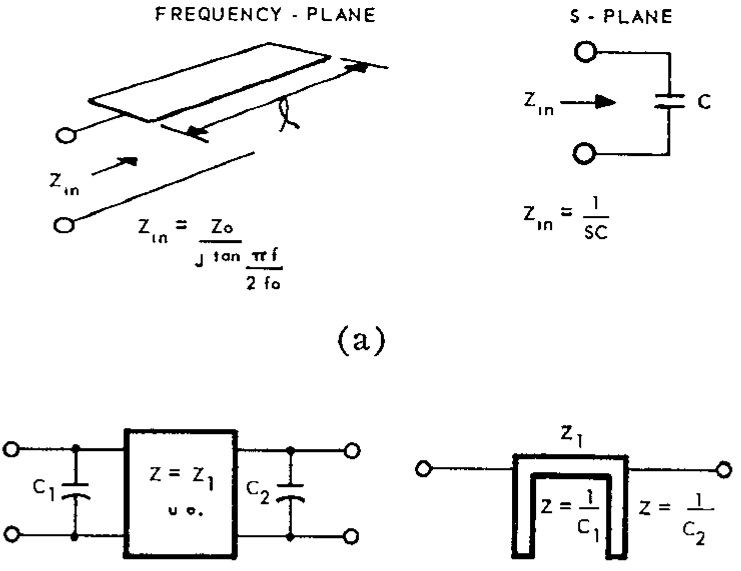
\includegraphics[width=\imagewidth]{images/bereich}
    \caption{Auszug aus \cite{ref:wenzel}: (a) Realisierung einer Kapazit\"at als Stichleitung, (b) Netzwerk in der S-Ebene, (c) Realisierung der Stichleitung}
    \label{fig:bereich}
\end{figure}

Betrachtet  man als Beispiel  ein  einfaches  TEM-Netzwerk  einer  Kapazit\"at
(siehe Abbildung \ref{fig:bereich}), sieht man, dass die  Wellenimpedanz $Z_0$
von  der Kapazit\"at $\frac{1}{C}$ abh\"angt. W\"urde man  die  Wellenimpedanz
$Z_0$ in Funktion der L\"ange $l$ plotten, so w\"urde man schnell feststellen,
dass f\"ur $Z_0<10$ die Leitungsst\"ucke sehr breit werden und  f\"ur  $Z_0  >
300$ die Leitungsst\"ucke sehr schmal werden.

Der Umsetzbare Bereich von $Z_0$ und  somit  von  $C$  ist  also  nur  in  der
Gr\"ossenordnung von $1:30$ m\"oglich. Die Realisierbarkeit eines arbitr\"aren
Frequenzgangs    kann    zum    teil   schwierig   oder   unm\"oglich    sein.
Gl\"ucklicherweise gibt es  mehrere  physikalische Umsetzungen die das gleiche
Verhalten aufweisen.  Es  ist  also  von  Vorteil,  wenn man bei der Umsetzung
mehrere L\"osungen betrachtet.

> Recht tricky sich in ein solch spezifischen Gebiet einzuschaffen. 
> Interessant zu sehen, dass es andere Orte gibt, wo Transformationen verwendet werden (also nicht nur bei digitalen Filtern, sondern bie der Hf-Technik und es eindrücklich ist, wie ähnlich sie sind)
> Überblick zu halten ist recht schwierig.
> Interessant, neue Tools und deren Anwendung kennenzulernen.

